\chapter{Turbulent transport}
\label{chap:TransportTurbulent}

The charge density fluctuations around Boltzmann distribution are inherent to plasmas. They are on a scale shorter than the Debye length since a charged particle is sensitive only to other particles within its Debye sphere. Here it will be shown that charge density perturbations can occur on a larger scale. We will take as an example the drift wave, a typical instability in the confined plasma, but we could also consider the interchange instability. These perturbations contribute to plasma transport, which will be discussed with the help of the electric drift around the electrostatic potential extrema.

There are several possible frameworks to study the effect of turbulence on transport. The gyrofluid theory can be developed by solving the equations formed as the first moments of Vlasov's equation (averaged over the cyclotron motion) to which is added a closure relation. It is also possible to develop the gyrokinetic theory, which consists in looking for the distribution function response to a perturbation (again with an average over the cyclotron motion). For either of these two models, the theoretician can choose to study the linear plasma response to a weak perturbation - it is the quasilinear approach. It is also possible to include the interactions of the various quantities with each other - this is the nonlinear approach. A number of ingredients can be added to the model, such as the finite Larmor radius effects, various kinds of collision operators... The nonlinear gyrokinetic approach has two versions: the so-called 'local', which calculates only the deviation to the equilibrium distribution function and the so-called 'full-f' which consists in calculating the complete distribution function. The choice of the framework depends on the specific problem to be studied, on the desired accuracy and on the available computation time.

These various models will not be described in detail here but we will use one or the other depending on the specific point discussed.



		\section{Effect of fluctuations on a test particule}
		\label{sec:FluctuationsParticuleTest}
		
				\subsection{Fluctuations of the magnetic field}
				\label{FluctuationsDuChampMagnetique}

Let us make the approximation of a particle submitted to turbulence in a plasma tokamak witouht having any influence on it, as is the case when trace impuities are injected into a plasma for a transport study.

If the magnetic field $\vec{B}$  fluctuates around an average field $\vec{B}_{eq}$:
\[
		\vec{B} = \vec{B}_{eq} + \tilde{\vec{B}},
\]

The direction of the particle guiding centre, which is always aligned with the total field, will be submitted to small deviations. For instance, in the radial direction (which is still the one we are interested in), the fluctuating part of the particle velocity is given by:
\[
		\tilde{v}_r = \frac{\tilde{B}_r}{B_{eq}}v_\|
\]
The resulting radial displacement, of which the scale is denoted $\Delta$:
\[
		\Delta^2 \simeq \left< |\tilde{v}_r|^2\!\right>\tau_{c\|} = \left< \left| \frac{\tilde{B}_r}{B_{eq}} \right|^2\right> \lambda_{c\|}^2
\]
Here $\tau_{c\|}$, which is called the correlation time, is the time during which the particle is submitted to the fluctuation and $\lambda_{c\|}$, called the correlation length, is the corresponding distance in the parallel direction. If the particle is fast or if the fluctuation lifetime is long, $\lambda_{c\|}$ is the characteristic length of a $B$ fluctuation in the radial direction. On the contrary if the particle is slow or if the fluctuation lifetime is short, $\lambda_{c\|}$  is the distance travelled by the particle in the parallel direction during time $\tau_{c\|}$. In both cases, we have $\lambda_{c\|} = v_\|\tau_{c\|}$. 

An order of magnitude of the diffusion coefficient can be obtained by writing:
\[
		D_M \simeq \frac{\Delta^2}{\tau_{c\|}} = \left< \left| \frac{\tilde{B}_r}{B_{eq}} \right|^2\right> \lambda_{c\|} v_\|
\] 
This expression shows that diffusion due to the magnetic field fluctuations increases with velocity. It is thus stronger for electrons than for ions. Assuming that $\lambda_{c\|}$ is of the same order as the transit length and that the parallel velocity is equal to the thermal velocity, we have:
\[
		D_M \simeq \pi q R v_{th,e} \left< \left| \frac{\tilde{B}_r}{B_{eq}} \right|^2\right>
\]
and, with reasonable values of $q$, $R$ and $T_e$:
\[
		D_M \simeq 10^8 \left< \left| \frac{\tilde{B}_r}{B_{eq}} \right|^2\right>		\mbox{(en m$^2$/s)},
\]
which gives 1 m$^2$/s for magnetic field fluctuations of 10$^{-2}$\%.
		
		
				
				\subsection{Fluctuations of the electrostatic field}
				\label{FluctuationsDuChampElectrostatique}
		
		
Let us assume now that the fluctuations are of an electrostatic nature. The electrostatic potential will be denoted $\phi = \tilde{\phi}$ assuming that the equilibrium potential is 0 (which is true for scales longer than the Debye length.) The test particle drifts around the potential extrema because of the electric drfit:
\[
		\tilde{\vec{v}}_E = \frac{\tilde{\vec{E}} \times \vec{B}}{B^2}
\]
of which the radial projection is:
\[
		\tilde{v}_{Er} = \frac{\tilde{E}_{\theta}}{B}
\]
The radial distance travelled by the particle during the parallel correlation time is of the order of $\Delta$:
\[
		\Delta^2 = \left< |\tilde{v}_{Er}|^2\right>\tau_{c\|}^2
\]
From this we can deduce an order of magnitude of the coefficient diffusion associated with electrostatic turbulence:
\[
		D_{ES} \simeq \frac{\Delta^2}{\tau_{c\|}} = \left< \left| \frac{\tilde{E}_\theta}{B} \right|^2 \right> \lambda_{c\|}/v_\|
\]
In this case diffusion is stronger for slow particles, i.e. ions.

By definition we have $\tilde{E} = -\nabla \tilde{\phi}$ and assuming that the turbulence scale in the poloidal direction is characterised by $1/k_\theta$ we get that $\tilde{E}_\theta \simeq k_\theta \tilde{\phi}$. In addition, we can express the magnetic field as a function of the thermal velocity and the ion Larmor radius:
\[
		\frac{1}{B} = \frac{e\rho_i}{mv_{th,i}}
\] 
The diffusion coefficient associated with electrostatic turbulence can thus be expressed in the following way:
\[
		D_{ES} \simeq \pi q R v_{th,i}(k_\theta \rho_i)^2 \left< \left| \frac{e \tilde{\phi}}{T} \right|^2 \right>
\]
or, with reasonable values of the plasma quantities:
\[
		D_{ES} \simeq 10^4 \left< \left| \frac{e \tilde{\phi}}{T} \right|^2 \right>		\mbox{(en m$^2$/s)}.
\]
This ives a diffusion coefficient of 1 m$^2$/s for electrostatic potential fluctuations of 1\%. 

For a comparable diffusion coefficient, the relative level of electrostatic fluctuations must be much higher than that of magnetic fluctuations (two orders of magnitude). However anomalous transport (i.e. the difference between observed transport and the neoclassical predictions) is usually explained by the former, on the one hand because magnetic fluctuations even of a low level are hard to justify and on the other hand because the elctrostatic fluctuation level measured in tokamaks is of the order of 1\% in the centre and more than 10\% (even 100\%) at the edge. In the following, only the electrostatic potential fluctuations will be discussed.

		\section{Diffusion Quasi-linear electrostatic turbulent diffusion}
		\label{sec:DiffusionQuasiLineaire}
		
		
In Section \ref{sec:FluctuationsParticuleTest}, a relation was obtained between the turbulent diffusion coefficient and the plasma characteristics for a test particle. We are now going to look for the global plasma response assuming that the plasma responds linearly to an electrostatic potential perturbation.This situation corresponds to a 'weak' perturbation of which the average is 0 over a time long compared with the perturbation evolution time (generally called the turbulence correlation time).

As in all that has been discussed above, only the flux radial component will be considered (the other components are generally 0).We do not know its expression but the drift velocity dcalculations allow us to write the component perpendicular to the magnetic field (which contains the radial component):
\[
		\vec{\Gamma}_\perp = n \left( \vec{v}_E + \vec{v}_{dia} + \vec{v}_{pol} \right)
\]

The radial flux is the radial component of the perpendicular flux: $\Gamma_r = (\Gamma_\perp)_r$. The radial turbulent flux is the time average of this instantaneous radial flux over a time long compared with the turbulence correlation time $\tau_c$:
\[
		\vec{\Gamma}_{r,turb} = \left< \vec{\Gamma}_r \right> = \left< n \vec{v}_r \right>
\]
where $\left<...\right>$ represents the time average. these quantities are of course averages over a flux surface, i.e. over angles $\theta$ and $\varphi$.

The polarisation velocity $\vec{v}_{pol}$ is in the perpendicular direction, and its intensity is of the order of $\rho_L / L_c$ where $\rho_L$  is the Larmor radius and $L_c$ is the turbulence correlation length. The velocity $v_{pol}$ is thus significant only when $L_c$ is small, which corresponds to a situation of small scale turbulence which contributes little to transport. The effect of $v_{pol}$ will thus be neglected. We are left with:

\[
		\vec{\Gamma}_{r,turb} = \left< n \vec{v}_{Er} \right> + \left< n \vec{v}_{dia,r} \right>
\]
By taking the known expression of the diamagnetic drift velocity, we obtain:
\begin{eqnarray*}
		\left< n \vec{v}_{dia,r} \right>	&	=	&	\left< \frac{\left(\vec{B} \times \vec{\nabla}p \right)_r}{eB^2} \right>			\\
																			&	=	&	\frac{ \left( \vec{B} \times \left< \vec{\nabla}p \right> \right)_r }{eB^2}		\\
																			&	=	&	\left< \frac{\left(\vec{B} \times \vec{\nabla}p_{eq} \right)_r}{eB^2} \right>
\end{eqnarray*}
since the time average of the fluctuating pressure gradient is 0: $\left< \nabla \tilde{p} \right> = 0$. As the equilibrium pressure gradient is in the radial diractione, the diamagnetic drift velocity contribution to the turbulent flux is 0. Only the electric drift velocity contribution remains:
\[
		\vec{\Gamma}_{r,turb} = \left< n \vec{v}_{Er} \right>
\]

We are now going to use the quasilinearity assumption: we assume that the plasma quantities respond to a weak fluctuating perturbation by a weak fluctuating perturbation:
\begin{eqnarray*}
		n	&	=	&	n_{eq} + \tilde{n}		\\
		\vec{v}	&	=	&	\vec{v}_{eq} + \tilde{\vec{v}}		\\
		p	&	=	&	p_{eq} + \tilde{p},		\\
		\ldots	&	&
\end{eqnarray*}
We can re-write the total average flux:
\begin{eqnarray*}
		\vec{\Gamma}_r	&	=	&	\left< n_{eq} \vec{v}_{Er,eq} \right> + \left< \tilde{n} \tilde{\vec{v}}_{Er} \right>	\\
											&	=	&	n_{eq} \vec{v}_{Er,eq} + \left< \tilde{n} \tilde{\vec{v}}_{Er} \right>		\\
											&	=	&	\vec{\Gamma}_{r,eq} + \vec{\Gamma}_{r,turb}
\end{eqnarray*}
The dirst term is the equilibrium flux (i.e. over a time scale longer than the fluctuation time scale) and the second term is the radial flux associated with turbulence.

Before giving this flux expression, we are going to use the continuity equation to obtain the density response to this turbulent flux:
\[ 
		\frac{\partial n}{\partial t} + \vec{\nabla}.\vec{\Gamma}_r = 0
\]
Using the linearity assumption, we get:
\begin{eqnarray*}
		\frac{\partial n_{eq}}{\partial t} + \vec{\nabla}.\vec{\Gamma}_{r,eq} & = & 0		\\
		\frac{\partial \tilde{n}}{\partial t} + \vec{\nabla}.\vec{\Gamma}_{r,turb} & = & 0
\end{eqnarray*}
and thus:
\[
		\frac{\partial \tilde{n}}{\partial t} + \left< \tilde{\vec{v}}_{Er}. \vec{\nabla} \tilde{n} \right> + \left< \tilde{n} \vec{\nabla}. \tilde{\vec{v}}_{Er} \right> = 0
\]

\begin{itemize}
\item In the case of a homogeneous $B$ field, we have:
\[
		\vec{\nabla}\vec{v}_E = \vec{\nabla}. \left( \frac{\vec{B}\times\vec{\nabla}\phi}{B^2} \right) = - \vec{\nabla}. \left( \vec{\nabla} \times \left( \frac{\phi \vec{B}}{B^2} \right) \right) = 0
\]
\item In the case of an inhomogeneous $B$ field, we have:
\[
		\vec{v}_E = - \vec{\nabla} \times \left( \frac{\phi \vec{B}}{B^2} \right) + \phi \frac{\vec{\nabla}\times \vec{B}}{B^2}
\]
and thus
\[
		\vec{\nabla}. \vec{v}_E = \vec{\nabla}. \left( \phi \frac{\vec{\nabla} \times \vec{B}}{B^2} \right) = \vec{\nabla} \phi . \frac{\vec{\nabla} \times \vec{B}}{B^2}
\]
In the frame moving with speed $\vec{v}_{E,eq}$, both factors of the right hand side member are small. Indeed,  $\nabla \phi = \nabla \tilde{\phi}$ is small and $\vec{\nabla} \times \vec{B}/B$ is of the order of $1/R$. We tus neglect $\vec{\nabla}. \vec{v}_E$.
\end{itemize}
The continuity equation has thus two terms left:
\[
		\frac{\partial \tilde{n}}{\partial t} + \left< \tilde{\vec{v}}_E . \vec{\nabla}\tilde{n} \right> = 0
\]

Any perturbation can be written in the form of a Fourier series:

\begin{eqnarray*}
		\phi & = & \sum_{m,n,\omega} \phi_{m,n,\omega}(r) e^{i(m\theta + n\varphi-\omega t)}		\\
		n   & = & \sum_{m,n,\omega}    n_{m,n,\omega}(r) e^{i(m\theta + n\varphi-\omega t)}		\\
\end{eqnarray*}
which can also be written:
\begin{eqnarray*}
		\phi & = & \sum_{\vec{k},\omega} \phi_{\vec{k},\omega}(r) e^{i(\vec{k}\vec{x}-\omega t)}		\\
		n   & = & \sum_{\vec{k},\omega}    n_{\vec{k},\omega}(r) e^{i(\vec{k}\vec{x}-\omega t)}		\\
\end{eqnarray*}
with $k_\theta = m/r$ (we will not have to deal with the toroidal dimension in this calculation).

Since $\tilde{\phi}$ and $\tilde{n}$ are physical quantities (and thus real), the Fourier coefficients must verify the relation:
\begin{eqnarray*}
		\phi_{-\vec{k},-\omega} & = & \phi_{\vec{k},\omega}^*		\\
		n_{-\vec{k},-\omega} & = & n_{\vec{k},\omega}^*
\end{eqnarray*}

If $B$ is homogeneous, the fluctuating electric drift velocity becomes:
\begin{eqnarray*}
		\tilde{v}_{Er} & = & \left( \frac{\vec{B} \times \vec{\nabla}\tilde{\phi}}{B^2} \right)_r	\\
									 & = & -\frac{1}{B^2}. B.\left( \nabla \tilde{\phi} \right)_\theta = - \frac{1}{rB}\frac{\partial\tilde{\phi}}{\partial\theta},
\end{eqnarray*}
or, using the Fourier development of $\phi$:
\[
		\tilde{v}_{Er} = \sum_{\vec{k},\omega} \left( -\frac{ik_\theta}{B} \right) \phi_{\vec{k},\omega} e^{i(\vec{k}\vec{x}-\omega t)}
\]
The turbulent flux expression thus becomes:
\begin{equation}
		\vec{\Gamma}_{r,turb} = \left< \tilde{n} \tilde{v}_{Er} \right> = \sum_{\vec{k},\omega} \left( -\frac{ik_\theta}{B} \right) n_{-\vec{k},-\omega} \phi_{\vec{k},\omega},
	\label{eq:flux_turb_prov}
\end{equation}
the time average of the other terms being 0. 

The continuity equation will provide a relation between the Density Fourier coefficients and the potential ones. Without time average, it has the following form:
\[
		\frac{\partial \tilde{n}}{\partial t} + \tilde{\vec{v}}_{Er}.\vec{\nabla}n_{eq} = 0.
\]

We have neglected the term $\tilde{\vec{v}}_{E,eq}.\vec{\nabla}\tilde{n}$, which is of second order, and we have chosen the frame moving at speed $\vec{v}_{E,eq}$, so that $\vec{v}_{E,eq}.\vec{\nabla}\tilde{n} = 0$. In the Fourier space, the equation becomes:
\[
		-i\omega n_{\vec{k},\omega} = -\frac{ik_\theta}{B} \phi_{\vec{k},\omega}.\nabla n_{eq},
\]
or:
\[
		n_{\vec{k},\omega} = \frac{k_\theta}{\omega B} \phi_{\vec{k},\omega}.\nabla n_{eq}
\]
which we replace in Eq. \ref{eq:flux_turb_prov}:
\[
		\Gamma_{r,turb} = - \sum_{\vec{k},\omega} \frac{i}{\omega} \left| \frac{k_\theta}{B}\phi_{\vec{k},\omega} \right|^2 \nabla n_{eq}
\]

It is possible to show that the divergence at $\omega = 0$ comes from the fact that we have neglected the second order term $\tilde{\vec{v}}_{E,eq}.\vec{\nabla}\tilde{n}$. If it is taken into account, instead of a divergence we have a resonance of which the width is often denoted $\Delta\omega_k$. The flux expression takes the new form:
\[
		\Gamma_{r,turb} = - \sum_{\vec{k},\omega} \frac{i\omega + \Delta\omega_k}{\omega^2+\Delta\omega_k^2} \left| \frac{k_\theta}{B}\phi_{\vec{k},\omega} \right|^2 \nabla n_{eq}
\]
This expression has the form of Fick's law with a diffusion coefficient:
\[
		D_{turb} = \sum_{\vec{k},\omega} \frac{i\omega + \Delta\omega_k}{\omega^2+\Delta\omega_k^2} \left| \frac{k_\theta}{B}\phi_{\vec{k},\omega} \right|^2
\]

The proportionality between $D_{turb}$ and $\left| \phi_{\vec{k},\omega} \right|^2$ indicates that diffusion is larger for modes with a large amplitude. The quasilinear framework does not provide quantitative results on the transport coefficients. Indeed it does not allow to calculate the electrostatic potential fluctuations ( which are necessary to know the Fourier coefficients $\phi_{\vec{k},\omega}$ and the $k_\theta$ spectrum of turbulence) in physical units. Only the nonlinear theory allows a complete calculation of the flux and the associated transport coefficients.



		\section{Phase and transport}
		\label{sec:DephasageEtTransport}
		
				\subsection{General case}
				\label{sub:DephasageCasGeneral}
				
We have seen in the previous section that the turbuent particle flux can be written:
\[
		\Gamma_{r,turb} = \left< \tilde{n}\tilde{v}_{Er} \right>_{t,\theta,\phi}
\]
where $\tilde{v}_{Er}$ is the radial component of the electric drift velocity and where the flux surface average is apparent. The electric drift velocity has the form $\tilde{v}_E = \tilde{E}_\theta/B$. As a result we have $\Gamma_{r,turb} = 0$ if $\tilde{n}$ and $\tilde{E}$ (or equivalently $\tilde{\phi}$) are in phase. To be more accurate, let us write the perturbed electrostatic potential and the density response as Fourier series:
\begin{eqnarray*}
		\tilde{\phi}  &  =  &  \sum_m \hat{\phi}_m e^{i\left( m\theta + \varphi_m^\phi \right)}		\\
		\tilde{n   }  &  =  &  \sum_m \hat{n}_m e^{i\left( m\theta + \varphi_m^n \right)}	
\end{eqnarray*}
(the toroidal dependence does not appear for the sake of simplicity, but it can be calculated in the same way), where the coefficients $\hat{\phi}_m$ et $\hat{n}_m$ are real and:
\begin{eqnarray*}
		\hat{n}_m     &  =  &  \hat{n}_{-m}			\\
		\hat{\phi}_m     &  =  &  \hat{\phi}_{-m}			\\
		\hat{\varphi}_m  &  =  &  - \hat{\varphi}_{-m}
\end{eqnarray*}
to ensure that $\tilde{\phi}$ and $\tilde{n}$ are real. The turbulent flux becomes:
\begin{eqnarray*}
		\Gamma_{r,turb}  &  =  &  \sum_m i \left( \frac{m}{rB} \right) \hat{n}_m \hat{\phi}_{-m} e^{i \left( \varphi_m^n + \varphi_{-m}^\phi \right)}		\\
										 &  =  &  \sum_m \left( \frac{im}{rB} \right) \hat{n}_m \hat{\phi}_m e^{i \left( \varphi_m^n - \varphi_m^\phi \right)}		\\
										 &  =  &  \sum_{m>0} \left( \frac{2im}{rB} \right)\hat{n}_m \hat{\phi}_m \sin \left( \varphi_m^n - \varphi_m^\phi \right)
\end{eqnarray*}
The resulting turbulent flux is finite if and only if $\varphi_m^n - \varphi_m^\phi \neq 0$, which means if at least one of the Fourier contibutions is out of phase. As a consequence, the assumption of an adiabatic electron response  ($\tilde{n}/n_{eq} = e\tilde{\phi}/T_e$) does not produce any radial turbulent flux.


				\subsection{Drift wave}
				\label{OndeDeDerive}
				
				
\begin{figure}[htbp]
	\centering
		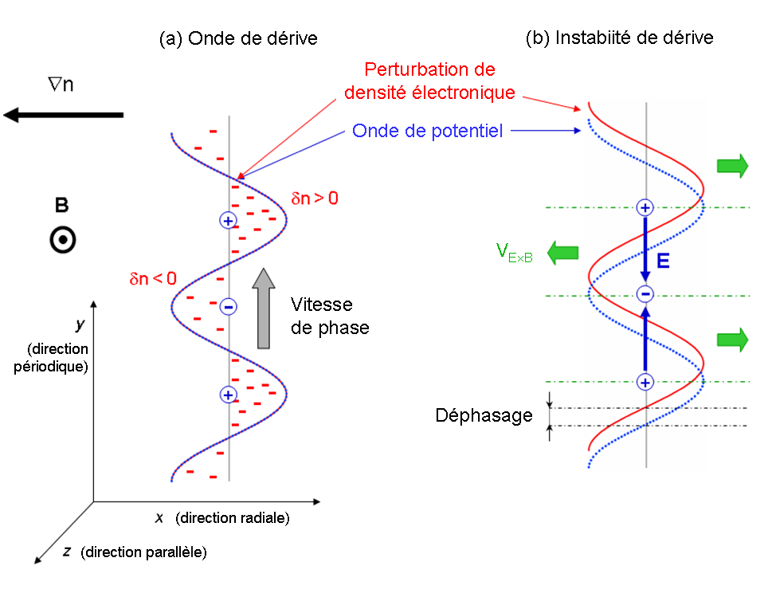
\includegraphics[width=0.70\textwidth]{Fig_onde_de_derive.png}
	\caption{Schematic representation (a) of a drift wave propagating in the poloidal direction, (b) of a drift instability driving transport).}
	\label{fig:onde_de_derive}
\end{figure}

The drift wave allows to give an example of a situation where the density response is ou of hpase with respect to the fluctuating potential excitation. Let us consider at a given time a periodical perturbation of the electrostaticpotential in the poloidal direction (denoted $y$ on the figure): $\tilde{\phi} \propto \exp{i \left( k_y y - \omega t \right)}$. If the perturbation frequency is not too large, the electron distribution adapts instantaneously to the potntial and the electron density fluctuation is in phase with that of the potential. This is called the electron adiabaticity hypothesis. The result is shown in Fig. \ref{fig:onde_de_derive}.a: over-density zones around the potential maxima alternate with under-density zones around the potential minima.
				
Let us look now at the electric drift velocities of the various zones in this simplemodel. By definition, the electric field $E_y$ is directed from the potential maxima to the potential minima, hence from the overdensity zones to the under-density zones. Taking into account the direction of $\vec{B}$ as indicated on the figure, we see that the upper (on the figure) half of an over-density zone is submitted to an outward drift, whereas the lower half is pushed inward. In the same way, the upper half of an under-density zone is pushed inward whereas the lower half is pushed outward. The global effect is the perturbation propagation in the poloidaldirection ($y$ on the figure), without amplification or damping. There is no transport in this case, which is in agreement with the result of the previous paragraph.

In the case where the density response is out of phase with the potential fluctuation (Fig. \ref{fig:onde_de_derive}.b), the symmetry between the zones pushed inward and outward is broken. The global effect is indeed that of electron trnasport. Depending on the sign of the phase sift, the phenomenon is stabilising (if the over-density zones are pushed inward and the under-density zones are pushed outward) or destabilising (in the opposite case).

\textit{Exercise: is the situation shown in Fig. \ref{fig:onde_de_derive}.b stabilising or destabilising?}

A poloidally periodic perturbation of the potential can thus be ineffective for transport (if density and potential are in phase), damped or responsible for a macroscopic transport. This third situation is the object of turbulent transport modelling.

Phase shifts between potential and density can be due to resistivity, which invalidates the electron adiabaticity hypothesis, or to resonances between wavec and particles.

		
		\section{A few propoerties of the quasilinear theory}
		\label{sec:QuelquesProprietesDeLaTheorieQuasiLineaire}
		
				\subsection{Resonance and Landau damping}
				\label{sub:ResonanceEtAmortissementDeLandau}
				
				
In the previous discussion we have used the fluid model. Now we are going to give a gyrokinetic description of the plasma. it is now described by the guiding centre distribution function, generaly denoted $f$, in the phase space. To make the developments  simpler, we will use a two dimension phase space: one for position ($r$) and one for velocitiy ($V$). With the appropriate normalisations, Vlasov's and Poisson's equations take the following forms:
\begin{eqnarray*}
		\partial_\tau f + V \partial_x f + \partial_x \phi \partial_V f = 0		\\
		\partial_x^2 \phi = \int_{-\infty}^{+\infty} f dV - 1
\end{eqnarray*}
où $\partial_a = \partial/\partial a$ et où les normalisations adoptées sont les suivantes:
\begin{eqnarray*}
		x     &  =  &  \frac{r}{\lambda_D} = \sqrt{\frac{n_e e^2}{\epsilon_0 k_B T}}r		\\
		\tau  &  =  &  \omega_{pe} t = \frac{v_{th,e}}{\lambda_D} t											\\
		V			&  =  &  \frac{v}{v_{th,e}}			\\
		\phi  &  =  &  \frac{e\Phi}{T_e}
\end{eqnarray*}
where $\Phi$ is the electrostatic potential in physical units. In addition, $f$ is normalised to $v_{th,e}/n_e$ (instead of 1).

At equilibrium (i.e. without fluctuating potential):
\[
		\partial_\tau f_{eq} = 0 \mbox{\hspace{1cm} et  \hspace{1cm}}  \phi = 0.
\]
Vlasov's equation thus becomes $\partial_x f_{eq} = 0$: $f_{eq}$ is a function only of $v$. Poisson's equation gives:
\[
		\int_{-\infty}^{+\infty} f_{eq} dv = 1
\]
The distribution function is now perturbed (weakly):
\[
		f(x,V,\tau) = f_{eq}(V) + \tilde{f} (x,V,\tau)		\mbox{\hspace{1cm} et  \hspace{1cm}}		\left< \tilde{f} \right>_{t,r} = 0
\]
Let us write Vlasov's equation again:
\[
		\partial_\tau f_{eq} + \partial_\tau \tilde{f} + V \partial_x f_{eq} + V \partial_x \tilde{f} + \partial_x\phi \partial_V f_{eq} + \partial_x\phi \partial_V \tilde{f} = 0
\]
The first and third terms are 0 for obvious reasons. The last term is of the second order and thus negligible. We are thus left with:
\[
		\partial_\tau \tilde{f} + V \partial_x \tilde{f} + \partial_x\phi \partial_V f_{eq} = 0
\]
Poisson's equation gives also some information:
\begin{eqnarray*}
		\partial_x^2\phi  &  =  &  \int_{-\infty}^{+\infty} f_{eq} dV  + \int_{-\infty}^{+\infty} \tilde{f} dV -1 \\
											&  =  &  \int_{-\infty}^{+\infty} \tilde{f} dV
\end{eqnarray*}

The plane wave functions are solutions of these equations. We are thus going to look for solutions which are linear combinations of plane waves:
\begin{eqnarray*}
		\tilde{\phi}		&		=		& \sum_{k,\omega} \hat{\phi}_{k,\omega} e^{i \left( kx - \omega \tau \right)}	\\
		\tilde{f}		&		=		& \sum_{k,\omega} \hat{f}_{k,\omega} e^{i \left( kx - \omega \tau \right)}
\end{eqnarray*}
With this type of solutions, Vlasov's and Poisson's equations give respectively:
\begin{eqnarray*}
		i\left( kV - \omega \right) \hat{f}_{k,\omega} + ik\hat{\phi}_{k,\omega} \partial_V f_{eq} = 0		\\
		-k^2\hat{\phi}_{k,\omega} = \int_{-\infty}^{+\infty} \hat{f}_{k,\omega} dV
\end{eqnarray*}
We deduce the following dispersion relation:
\begin{equation}
		k + \int_{-\infty}^{+\infty} \frac{\partial_V f_{eq}}{\omega - kV}dV = 0
\label{eq:dispersion}
\end{equation}
This relation is verified by the Vlasov's equation solutions.

The index $\epsilon(k,\omega)$ is defined in the following way:
\[
		\epsilon(k,\omega) = k + \int_{-\infty}^{+\infty} \frac{\partial_V f_{eq}}{\omega - kV}dV
\]
When $\omega$ is complex, the integration can be done using the residue theorem. When $\omega$  is real, it cannot be done due to the divergence in $\omega = kV$. Landau was the first to notice that it was necessary to make an analytic continuation so that the function $\epsilon(k,\omega)$ be defined even when $\omega$ is real:
\begin{equation}
		\epsilon(k,\omega) = k + P\int_{-\infty}^{+\infty} \frac{\partial_V f_{eq}}{\omega - kV}dV - \left( \frac{i\pi}{|k|}\partial_V f_{eq} \right)_{v=\omega/k}
\label{eq:ProlongementAnalytique}
\end{equation}
where the principal part is defined as:
\[
		P\int_{-\infty}^{+\infty} \frac{f(x)}{x-x_0}dx = \lim_{\epsilon\rightarrow 0}\left[ \int_{-\infty}^{x_0-\epsilon} \frac{f(x)}{x-x_0}dx + \int_{x_0+\epsilon}^{\infty} \frac{f(x)}{x-x_0}dx \right]
\]
The imaginary part of $\epsilon(k,\omega)$ is responsible for damping. This is called Landau damping. A development accompained by a few assumptions will allow us to know more precisely what this phenomenon is.

Let us assume that $\omega$ is 'weakly' complex, and separate the real part form the imaginary part:
\[
	\omega = \omega_r + i\omega_i, \mbox{ avec }	\omega_i << \omega_r
\]
If $\omega$ is a solution of the dispersion equation \ref{eq:dispersion}, we will have:
\[
	\epsilon = \epsilon_r  + i\epsilon_i, \mbox{ avec }	\epsilon_i << \epsilon_r
\]
We can develop $\epsilon$ to the first order:
\begin{eqnarray*}
	\epsilon(k,\omega) 	&	 \simeq  &  \epsilon(k,\omega_r) + i\omega_i \left( \frac{\partial\epsilon}{\partial\omega} \right)_{\omega = \omega_r}		\\
											&  \simeq  &  \epsilon_r(k,\omega_r) + i\epsilon_i(k,\omega_r) + i\omega_i \left( \frac{\partial\epsilon_r}{\partial\omega} \right)_{\omega = \omega_r}	- \omega_i \left( \frac{\partial\epsilon_i}{\partial\omega} \right)_{\omega = \omega_r}	\\
											&  \simeq  &  \epsilon_r(k,\omega_r) - \omega_i \left( \frac{\partial\epsilon_i}{\partial\omega} \right)_{\omega = \omega_r} + i\left[ \epsilon_i(k,\omega_r) + \omega_i \left( \frac{\partial\epsilon_r}{\partial\omega} \right) \right]_{\omega = \omega_r}
\end{eqnarray*}

The second term in the right hand side member of this equation can be neglected sinceit is of the second order. The dispoersion relation the imposes that:
\begin{eqnarray}
		\epsilon_r(k,\omega_r)  &  =  &  0		\nonumber\\
		\omega_i								&  =  &  - \frac{\epsilon_i(k,\omega_r)}{\left( \partial_\omega\epsilon_r \right)_{\omega_r}}		\label{eq:omega_i}
\end{eqnarray}

The equilibrium distribution function in a tokamak plasma is generally close to a maxwellian. we thus have:
\[
		f_{eq} = \frac{1}{\sqrt{2\pi}} e^{-v^2/2}
\]
With this distribution function, the index takes the following form:
\[
		\epsilon_r = k- \frac{1}{\sqrt{2\pi}} P \int_{-\infty}^{+\infty}\frac{v e^{-v^2/2}}{\omega-kv} dv
\]
from which we deduce:
\[
		\left( \frac{\partial \epsilon_r}{\partial \omega} \right)_{\omega=\omega_r} = \frac{1}{\sqrt{2\pi}}P \int_{-\infty}^{+\infty}\frac{v e^{-v^2/2}}{(\omega-kv)^2} dv
\]
In addition, the imaginary part of the index resulting from the analytic continuation (éq. \ref{eq:ProlongementAnalytique}) becomes:
\[
		\epsilon_i = \frac{\pi}{|k|}\frac{1}{\sqrt{2\pi}}\frac{\omega}{k} e^{-\frac{1}{2}\left( \frac{\omega}{k} \right)^2}
\]
We use Eq. \ref{eq:omega_i} to write the imaginary part of $\omega$:
\begin{eqnarray*}
		\omega_i  &  =  &   - \frac{\epsilon_i(k,\omega_r)}{(\partial_\omega \epsilon_r)_{\omega_r}}  \\
							&	 =  &	  - \frac{\pi}{|k|}\frac{1}{\sqrt{2\pi}}\frac{\omega_r}{k}e^{-\frac{1}{2}\left( \frac{\omega_r}{k} \right)^2} \times \frac{\sqrt{2\pi}}{P \int_{-\infty}^{+\infty} \frac{v e^{-v^2/2}}{(\omega_r-kv)^2} dv}
\end{eqnarray*}

Noticing that $v\times\exp(-v^2/2)$ is an odd function and that factor $1/(\omega_r-kv)^2$ is symmetrical with respect to $v = \omega_r/k$, we see that the principal part of the integral has the same sign as $\omega_r/k$. As a reuslt, $\omega_i$ is negative. The solution of the dispersion equation is thus a damped wave, independently from the effect of collisions.

The interpretation of this result is that the wave exchanges energy with the plasma particles. It is the fundamental mechanism of the wave-particle interaction, even in the case of turbulence.

NB: we have shown that $\omega_i <0$ in the case of a maxwellian. In the general case, the sign of  $\omega_i$ is that of $\partial_V f_{eq}$: if there exists a suprathermal partcle population, there can be a $v$ interval where $\partial_V f_{eq} > 0$, and thus $\omega_i >0$. The particles of which velocity is in this interval will thus be able to give away a part of their energy to a wave, which will then be amplified.


				\subsection{Resonance position and width}
				\label{sub:PositionEtLargeurDesResonances}

We have just discussed Landau damping in the velocity space. We are now going to look for the place where it occurs in the plasma.

We consider a tokamak plasma with a circular poloidal cross section and an infinite aspect ratio $R/a$.
The perturbation is again a plane wave $\exp i(m\theta + n\varphi)$ with wavelength large with respect to the ion Larmor radius.

The energy exchanged between the perturbing wave and the particles is:
\[
		W_{int} = 2\omega \mbox{Im}(\rho\phi^*)
\]
where $\rho$ is the charge density and $\phi$ the electrostatic potential.

The parallel wave vector $k_\|$ can be obtained with an order-of-magnitude reasoning:
\[
		\nabla_\| \simeq \frac{\vec{B}}{B}.\vec{\nabla} = \frac{1}{B}\left( B_\varphi. \nabla\varphi.\partial_\varphi + B_\theta.\nabla\theta.\partial_\theta \right) \simeq \frac{1}{R}\partial\varphi + \frac{1}{qR}\partial_\theta
\]
With the correspondances
\begin{eqnarray*}
		\partial_\varphi  &  \rightarrow	&  in	\\
		\partial_\theta   &  \rightarrow	&  im,	
\end{eqnarray*}
\[
\mbox{we obtain: } k_\| = \frac{1}{R}\left( n + \frac{m}{q} \right)
\]	
we have already seen elsewhere that $k_\theta = m/r$. In the vicinity $x$ of a radial position $r_{mn}$ such that $k_\| = 0$, or equivalently $q = - m/n$, or $k_\theta = m/r = -nq/r$, the exchanged energy has the form:
\[
		W_{int} = -\mbox{sgn}(\omega) W_0 \left| \frac{x_T}{x} \right| \left( \omega-\omega^*_n -\frac{\omega_T^*}{2} \left[ \left( \frac{x_T}{x} \right)^2 - 1 \right] \right)  \exp \left( - \frac{x_T^2}{2x^2} \right)
\]
where
\begin{eqnarray*}
		W_0  &  =  &  \sqrt{\pi} n_{eq} m_i v_T^2 \left| \frac{e\phi}{T_i} \right|^2		\\
		x_T  &  =  &  \frac{\omega L_s}{k_\theta v_T}			\\
		\omega_{n,T}  &  =  &  \frac{1}{2} \left( k_\theta \rho_i \right) v_{th} / L_{n,T}		\\
		L_s  &  =  &  \frac{qR}{s}
\end{eqnarray*}

The form of this function is shown in Fig. \ref{fig:Wint_résonance} (this figure is taken from Yanick Sarazin's lecture notes where the calculation is performed in a more detailed way).
\begin{figure}[htbp]
	\centering
		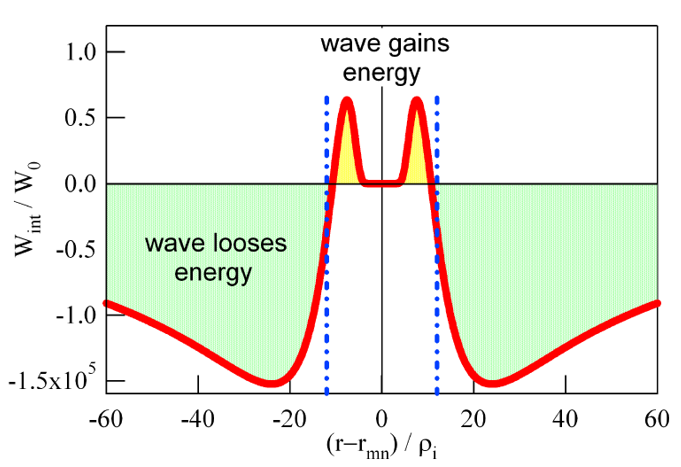
\includegraphics[width=0.70\textwidth]{Fig_Wint_resonance.png}
	\caption{Energy exchanged between a potential wave and the plasma particles as a function of the distance to a resonant surface}
	
	\label{fig:Wint_résonance}
\end{figure}
The most obvious result is that $W_{int}$ has well marked minima slightly beyond $x = x_T$ (values $x_T$ and $-x_T$ are indicated by vertical dashed lines). The negative values of $W_{int}$ at these positions indicate that the wave gives a large part of its energy away to the particlesz. The consequence of this loss is that the wave does not propagate beyond these minima. The interaction takes place in a region of width:
\[
		\Delta \simeq \frac{\omega}{\omega_T^*}\frac{L_s}{L_T}\rho_i
\]
around the so-called rational surfaces (i.e. characterised by a rational safety factor $q = m/n$). If the width $\Delta$ is smaller than the distance between rational surfaces $\Delta_r \simeq 1/k_{\theta s}$, the various modes are resonant in non-adjacent regions and thus cannot interact with each other. In the other case, they can transfer energy to each other through their exchanges with particles. On a macroscopic scale, this gives rise to transport. The boundary between these two regimes can be quantified with the Chirkov parameter:
\[
		\sigma_{Chir} = \frac{\Delta}{\Delta_r} = 1
\]
In a tokamak, we have in general $L_s \simeq 3$ m and $L_T \simeq 0,25$ m, and thus $\sigma_{Chir} > 1$. Tokamaks are in a regime where instabilities due to electrostatic potential fluctuations drive energy exchanges on the macrosopic scale. These exchanges are the expresion of turbulent transport.



		\section{Nature of turbulent modes: ITG, ETG and TEM}
		
As it was shown rapidly in the previous paragraph, the resonance condition refers to the fluctuation wavenumbers but also to a scale characteristic of the plasma particles. More specifically, if the characteristic scale of a particle type is large with respect to the wavelength of the considered mde, there is no interaction (no energy exchange): the particle population is adiabatic.

As a result, a categorisation of turbulent modes has been adopted. FThere are four classes of modes, related to the four types of plasma particles (passing and trapped electrons, passing and trapped ions, impurities being left aside since they are traces most of the time), of which the names are always referrred to in the turbulent transport studies.

They are the following, sorted by descending order of wavelength. The very large wavelength modes (larger than the ion banana width) are called TIM (\textit{Trapped Ion Modes}) because they interact with trapped ions. For wavelengths between the ion banana width and the ion Larmor radius, the modes are called ITG (\textit{Ion Temperature Gradient}) because they are destabilised when the ion temperature gradient is large (or equivalently when the gradient length is small compared with the plasma minor radius). For wavelengths between the ion Larmor radius and the electron banana width, the modes are called TEM (\textit{Trapped Electron Modes}). finally for wavelengths between the electron banana width and the electron Larmor radius, the modes are called ETG (\textit{Electron Temperature Gradient}).

In practice, the ion Larmor radius and the electron banana width are of the same order of magnitude. The ITG modes and  TEMs are thus present in the same wavelength range. The situation is sketched in Fig.  \ref{fig:_schéma_modes_turb}.
\begin{figure}[htbp]
	\centering
		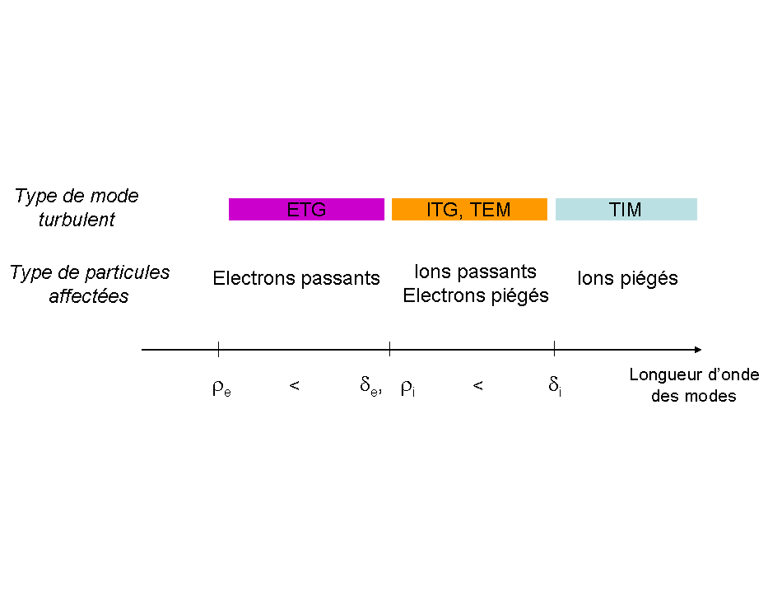
\includegraphics{Fig_schema_modes_turb.png}
	\caption{Turbulent mode classes a a function of wavelength. The type of particles interacting with the mode ins indicated.}
	\label{fig:_schéma_modes_turb}
\end{figure}

A detailed treatment shows that the ion type modes (ITG, TIM) rotate in the ion diamagnetic drift direction and the electron modes in the electron diamagnetic drift direction. It is one of the experimental tests which allwos to distinguish between ITG and TEM.

\textbf{NB 1:} The TIM modes, which could contribute to transport on a macroscopic scale, are never taken into account since their amplitude is weak.

\textbf{NB 2:} The ETG modes are small scale modes. Although always present, they contribute little to macroscopic transport. However, there are processes (not discussed in these notes) which allow these modes to transfer energy to longer wavelength modes. These processes coudl play an important role in improved confinement regimes, where large scale turbulence is strongly suppressed.





%		\section{Modèle du gradient critique}
		
		\section{Turbulent flux in the quasilinear theory}
		\label{FluxTurbulentsDansLaTheorieQuasiLineaire}

In order to determine the form of the turbulent particle and heat fluxes, we adopt the quasilinear gyrokinetic theory frame and we calculate the response $\tilde{f}$ of the distribution function to a perturbation $\tilde{H}$ of the hamiltonian. In general for $\tilde{H}$ an electrostatic potential perturbation is chosen. This a hypothesis of the model: we thus constrain the $k$ spectrum shape of turbulence as well as its amplitude. As a result, this model can be used to obtain the flux dependences on the plasma gradients but not their absolute values.

The fluxes take the well known form:
\[
	\Gamma_s = -D_s \nabla n_s + V_s n_s
\]
where the index $s$ stands for the particle type. The diffusion coefficient and the convection velocity are:
\begin{eqnarray*}
		D_s  &  =  &  \left( \frac{q}{rB} \right)^2 \sum_{n,\omega_0} n^2 \left< \sqrt{\frac{\xi}{\pi}} e^{-\xi}.\frac{\gamma_0}{\left( n\Omega_s(\xi,\lambda) - \omega_{r0} \right)^2 + \gamma_0^2} \right>_{\xi,\lambda} \left| \tilde{\phi}_n \right|^2		\\
		V_s  &  =  &  - C_s^{th} \frac{\nabla T_s}{T_s} + \frac{C_q^c}{R}
\end{eqnarray*}

The somewhat complicated expression of the diffusion coefficient does not allow to discuss easily the parameters on which it depends but the turbulent diffusion dependence on the squared modulus of the fluctuating potential is retrieved.

The convection velocity expression shows two terms. The first one,proportional to the normalised temperature gradient of the considered species is called thermodiffusion. The proportionality coefficient $C_s^{th}$ depends on $1/Z$ ($Z$ being the species charge). The electron thermodiffusive flux is thus in opposite direction of the ion and impurity flux. Calculations show that the direction of this thermodiffusive flux depends on the turbulence type. It is outward for electrons (inward for ions and impurities) when turbulence is of the electronic type and in the oppposite direction when turbulence is of the ion type.

The second term is called curvature term. It is the dominant term. The coefficient $C_q^c$ is porportional to the normalised $q$ gradient $\nabla q/q$. The resulting flux is directed inward if the magnetic shear $s$ is positive, and outward if $s$ is negative (the exact limit is not strictly 0 but a negative value between -1 and 0). An additional term is often included in the curvature term. It is called the parallel compressibility flux, which is small and in opposite direction with respect to the thermodiffusive flux.

%		\section{Tests expérimentaux}
		
%				\subsection{Mise en évidence des seuils}
				
%				\subsection{Rôle des gradients}
				
%				\subsection{Rôle de la charge des particules}
				
%				\subsection{Nature de la turbulence et renversement de convection}

